\documentclass[UTF8]{ctexart}

\usepackage{algorithm}
\usepackage{algorithmic}
\usepackage{amsmath,amssymb}
\usepackage{booktabs}
\usepackage{geometry}
\usepackage{tikz}
\usepackage{color}
\geometry{a4paper,scale=0.7}

\begin{document}
    SA22225226 李青航

    ~\\
    \noindent\textbf{475}

    \usetikzlibrary {graphs.standard}
    \tikz \graph {
    subgraph I_nm [V={a, b,c, d}, W={1,...,5}];

    a -- { 1, 2};
    b -- { 1, 2,3,4 };
    c -- { 1,2, 3, 4,5 };
    d -- { 3, 4, 5 };
    };

    ~\\
    \noindent\textbf{492}

    从左到右,从上到下,编号1,2,3,4……

    图一邻接矩阵
    $$
    \begin{bmatrix}
        0 & 1 & 1 & 0  \\
        1 & 0 & 1 & 1  \\
        1 & 1 & 1 & 1  \\
        0 & 1 & 1 & 0  \\
    \end{bmatrix}
    $$

    图二邻接矩阵
    $$
    \begin{bmatrix}
        0 & 1 & 1 & 0  \\
1 & 0 & 1 & 1  \\
1 & 1 & 0 & 1  \\
0 & 1 & 1 & 1  \\
    \end{bmatrix}
    $$

    ~\\
    \noindent\textbf{495}

    图(a)没有欧拉迹,因为有顶点的度为奇数,且奇数度顶点不是两个

    图(b)有欧拉闭迹,所有顶点的度都为偶数

    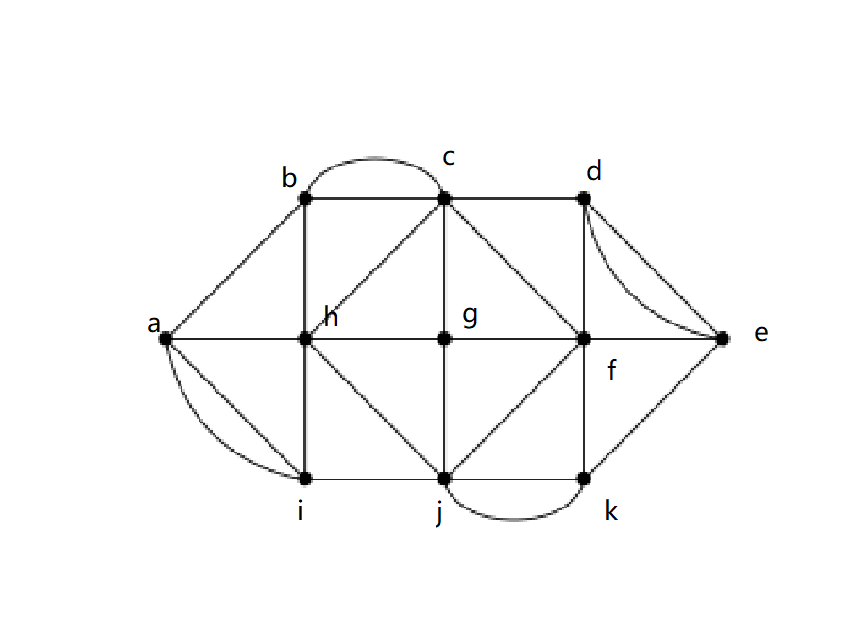
\includegraphics{1.png}

    先找一条闭迹$\gamma _1=a-i-a-b-c-b-h-a$ 

    再找一条闭迹$\gamma _2=h-i-j-k-j-h$

    再找一条闭迹$\gamma _3=h-c-g-j-f-g-h$

    再找一条闭迹$\gamma _4=c-f-k-e-d-e-f-d-c$

    合成$\gamma _1 \mathop{*}\limits ^{h} \gamma _2=a-i-a-b-c-b-h-i-j-k-j-h-a$
    
    再合成$\gamma _1 \mathop{*}\limits ^{h} \gamma _2 \mathop{*}\limits ^{h} \gamma _3= 
    a-i-a-b-c-b-h-c-g-j-f-g-h-i-j-k-j-h-a
    $

    再合成$\gamma _1 \mathop{*}\limits ^{h} \gamma _2 \mathop{*}\limits ^{h} \gamma _3
    \mathop{*}\limits ^{c} \gamma _4=
    a-i-a-b-c-f-k-e-d-e-f-d-c-b-h-c-g-j-f-g-h-i-j-k-j-h-a
    $

    ~\\
    \noindent\textbf{527}

    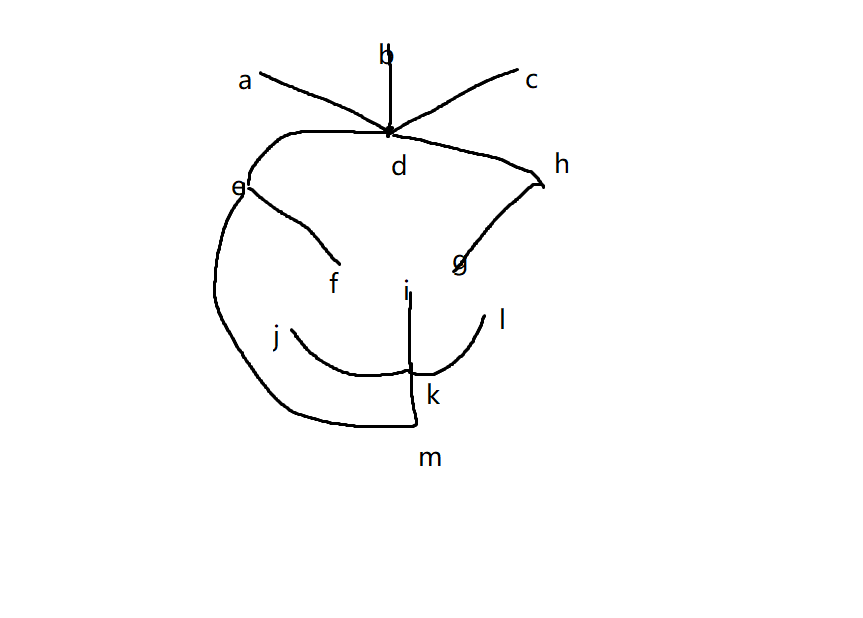
\includegraphics{2.png}

    ~\\
    \noindent\textbf{574}

    使用Theorem 12.1.9得到的是$\rho (t_1)=t_2, \rho (t_2)=t_3 ,
    \rho (t_3)=t_1$

    恰好是一个有向圈,都拿到了自己最喜欢的商品

    ~\\
    \noindent\textbf{578}

    第一个有向圈
    $\rho (t_1)=t_3, \rho (t_3)=t_5, \rho (t_5)=t_1$

    第二个$\rho (t_2)=t_4, \rho (t_4)=t_2$

    第三个$\rho (t_7)=t_7$

    第四个$\rho (t_6)=t_6$

\end{document}